% Sección "Materiales y métodos" alineada con la implementación real del
% repositorio. Requiere: graphicx, subcaption, booktabs, hyperref.

\section{Materiales y métodos}

\subsection{Conjunto de imágenes}

Para la evaluación se seleccionaron las imágenes Apollonian Gasket, Lena, Baboon y una imagen de un texto extraído del Arte de la Guerra de Sun Tzu. Las imágenes tienen todas un tamaño de $512\times512$ píxeles y se encuentran en los formatos PGM ASCII (P2)\cite{netpbmPGM}, PNG y JPEG, asegurando que todos los métodos partan exactamente del mismo contenido visual. Se definió utilizar estas dimensiones de modo que puedan aplicar a los tamaños de bloques evaluados.

PGM ASCII (P2) representa imágenes en escala de grises mediante valores de intensidad almacenados sin compresión. Este es el formato de entrada usado por el compresor. Las imágenes del experimento y las referencias PNG/JPEG están disponibles en el repositorio del trabajo detallado en la Sección~\ref{sec:entorno_ejecucion}.

\begin{table}[htbp]
\centering
\caption{Conjunto de imágenes utilizado en la evaluación experimental. El tamaño corresponde al archivo PGM ASCII de entrada.}
\label{tab:conjunto_imagenes}
\begin{tabular}{lcrc}
\toprule
Imagen & Dimensión & Tamaño (bytes) & Autosimilitud \\
\midrule
Apollonian Gasket & $512\times512$ & 1\,048\,134 & Alta \\
Lena & $512\times512$ & 966\,593 & Media \\
Baboon & $512\times512$ & 996\,517 & Baja \\
Sun Tzu & $512\times512$ & 1\,027\,181 & Baja (texto) \\
\bottomrule
\end{tabular}
\end{table}

\begin{figure}[htbp]
    \centering

    \begin{subfigure}[b]{0.23\textwidth}
        \centering
        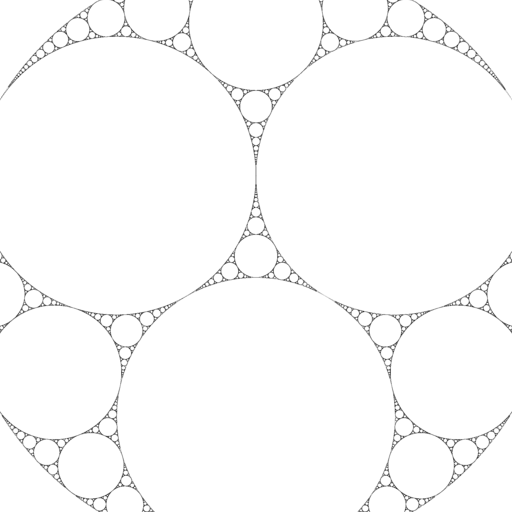
\includegraphics[
            width=\linewidth,
            trim=60 60 60 60,
            clip
        ]{images/apollonian_gasket_512.png}
        \caption{Apollonian Gasket}
    \end{subfigure}
    \hfill
    \begin{subfigure}[b]{0.23\textwidth}
        \centering
        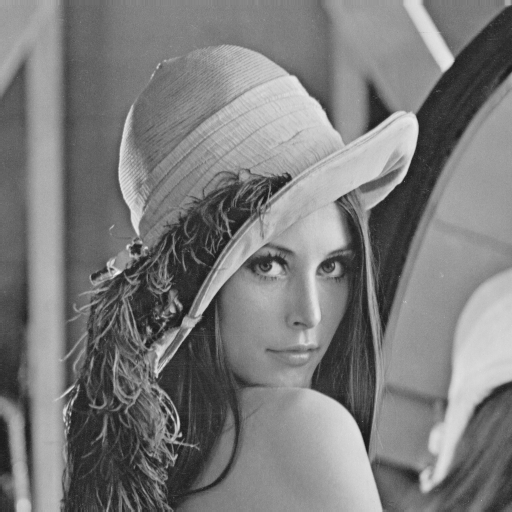
\includegraphics[width=\linewidth]{images/lena.png}
        \caption{Lena}
    \end{subfigure}
    \hfill
    \begin{subfigure}[b]{0.23\textwidth}
        \centering
        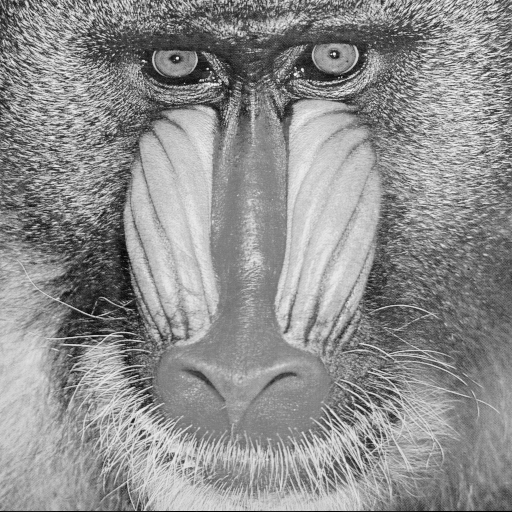
\includegraphics[width=\linewidth]{images/baboon.png}
        \caption{Baboon}
    \end{subfigure}
    \hfill
    \begin{subfigure}[b]{0.23\textwidth}
        \centering
        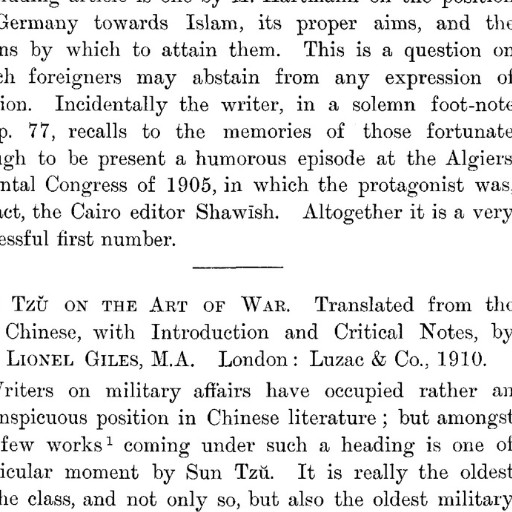
\includegraphics[width=\linewidth]{images/sun_tzu_512.png}
        \caption{Sun Tzu}
    \end{subfigure}

    \caption{Imágenes utilizadas en la evaluación experimental.}
    \label{fig:imagenes_evaluacion}
\end{figure}

\subsection{Clasificación de la autosimilitud}

La autosimilitud fue clasificada de manera perceptiva antes de realizar los experimentos. Para ello, se observaron la presencia de patrones repetitivos, regiones uniformes, texturas y bordes.

\begin{itemize}
    \item Alta: presencia clara de estructuras repetitivas (Apollonian Gasket).
    \item Media: presencia parcial de regiones semejantes (Lena).
    \item Baja: abundancia de texturas, bordes o estructuras poco repetitivas (Baboon).
    \item Baja (texto): predominio de tipografía y bordes agudos sobre fondo uniforme (Sun Tzu).
\end{itemize}

Sun Tzu se incluye como caso de contenido tipográfico, donde la autosimilitud geométrica entre bloques suele ser insuficiente para preservar la legibilidad de los caracteres.

\subsection{Configuración de los métodos}

Para la compresión fractal se utilizaron tres configuraciones:

\begin{itemize}
    \item Bloques rango de $4\times4$ y dominio de $8\times8$.
    \item Bloques rango de $8\times8$ y dominio de $16\times16$.
    \item Bloques rango de $16\times16$ y dominio de $32\times32$.
\end{itemize}

En los tres casos el bloque de dominio duplica el lado del bloque rango, por lo que la reducción al tamaño del rango se realiza con un factor $2{:}1$ mediante el promediado de vecindades de $2\times2$ píxeles. Los bloques rango forman una partición sin solapamiento de la imagen, y los bloques de dominio se toman de una grilla también sin solapamiento.

Se utilizaron ocho transformaciones geométricas básicas: identidad, rotaciones de $90^\circ$, $180^\circ$ y $270^\circ$, reflexiones horizontal y vertical, y reflexiones respecto de las dos diagonales. Para cada bloque rango se evaluaron todos los bloques de dominio reducidos combinados con las ocho transformaciones. Para cada par se calcularon los coeficientes de contraste $s$ y brillo $o$ por mínimos cuadrados, y se conservó la combinación de menor error cuadrático. Para la búsqueda no se aplicó ningún umbral máximo de error ni criterio de terminación anticipada, de modo que el costo de codificación es determinista y depende únicamente de la geometría de bloques.

Cada bloque rango queda descrito por la posición del dominio elegido, el índice de la transformación y el par $(s, o)$. El conjunto de estas asignaciones constituye el \emph{codebook} y es el artefacto que se mide como salida comprimida del método fractal, según se detalla en la Sección~\ref{sec:tamano_comprimido}.

La reconstrucción parte de una imagen inicial de ruido aleatorio y aplica de forma iterativa el sistema de funciones iteradas, lo que permite verificar que el punto fijo alcanzado no depende de la imagen de partida. La calidad se evaluó en las iteraciones 5, 10 y 20. Las iteraciones se indexan desde 0, por lo que las imágenes reportadas como iteración 5, 10 y 20 corresponden, respectivamente, a 6, 11 y 21 aplicaciones del operador de reconstrucción.

Para JPEG se evaluaron niveles de calidad de 25, 50, 75 y 90. Para PNG se utilizó compresión sin pérdida con la configuración predeterminada del codificador. El Cuadro~\ref{tab:referencias} resume los tamaños obtenidos por estas referencias.

\begin{table}[htbp]
\centering
\caption{Tamaño y bits por píxel de las referencias PNG y JPEG generadas a partir de los archivos PGM del experimento. PNG es sin pérdida. El número que acompaña a JPEG indica el nivel de calidad.}
\label{tab:referencias}
\scriptsize
\setlength{\tabcolsep}{2.5pt}
\begin{tabular}{lrrrrrrrr}
\toprule
& \multicolumn{2}{c}{Apollonian} & \multicolumn{2}{c}{Lena} & \multicolumn{2}{c}{Baboon} & \multicolumn{2}{c}{Sun Tzu} \\
\cmidrule(lr){2-3}\cmidrule(lr){4-5}\cmidrule(lr){6-7}\cmidrule(lr){8-9}
Formato & Bytes & bpp & Bytes & bpp & Bytes & bpp & Bytes & bpp \\
\midrule
PNG     & 23\,039 & 0,70 & 160\,263 & 4,89 & 210\,918 & 6,44 & 126\,887 & 3,87 \\
JPEG 25 &  9\,461 & 0,29 &  13\,581 & 0,41 &  31\,112 & 0,95 &  33\,157 & 1,01 \\
JPEG 50 & 12\,992 & 0,40 &  20\,913 & 0,64 &  48\,852 & 1,49 &  48\,442 & 1,48 \\
JPEG 75 & 17\,487 & 0,53 &  32\,559 & 0,99 &  73\,167 & 2,23 &  66\,431 & 2,03 \\
JPEG 90 & 25\,150 & 0,77 &  59\,252 & 1,81 & 119\,506 & 3,65 & 100\,905 & 3,08 \\
\bottomrule
\end{tabular}
\end{table}

\subsection{Implementación y entorno de ejecución}
\label{sec:entorno_ejecucion}

La implementación de la compresión fractal fue desarrollada en Java, con codificación y decodificación paralelizadas mediante un pool de hilos de tamaño configurable. Los archivos de referencia PNG y JPEG se generaron con la biblioteca Pillow (que utiliza \textit{libjpeg} y \textit{zlib}) a partir de los mismos archivos PGM empleados por el compresor fractal. El código fuente se encuentra disponible en el repositorio público del proyecto~\cite{madeoRepositorio}. Los experimentos se realizaron en la siguiente arquitectura: un procesador Apple M4 Pro de 12 núcleos con arquitectura \texttt{aarch64}, 24\,GiB de memoria RAM y macOS 15.1 (build 24B2082). Se utilizó OpenJDK 25.0.1, GraalVM CE 25.0.1+8.1 (HotSpot, modo mixto), con 12 hilos para la compresión y 12 para la descompresión.

Cada configuración se ejecutó una vez por imagen, sin calentamiento previo de la JVM, de modo que los tiempos reportados incluyen el costo de interpretación y de compilación JIT inicial. Por esta razón, los tiempos deben interpretarse como órdenes de magnitud comparativos entre configuraciones y no como mediciones de régimen estacionario.

\subsection{Medición del tamaño comprimido}
\label{sec:tamano_comprimido}

La salida del codificador fractal es un conjunto de asignaciones, una por bloque rango. Cada asignación requiere el índice del bloque de dominio seleccionado, el índice de la transformación aplicada y los coeficientes de contraste $s$ y brillo $o$. Si bien se almacena, la posición del bloque rango no se necesita. Las asignaciones se emiten en el orden de recorrido de la imagen, por lo que el bloque al que corresponde cada una queda determinado de forma implícita por su posición en la secuencia.

El costo de almacenamiento de cada asignación depende de cómo se serialicen esos campos. El archivo \texttt{.fc} que produce la implementación los guarda en representación textual, en la misma línea que el PGM ASCII (P2) de entrada, para que el lector pueda inspeccionar e interpretar el codebook sin herramientas adicionales. Esa decisión prioriza la legibilidad frente a la compactación. Existen formatos binarios o con cuantización de $(s,o)$ que ocuparían mucho menos espacio y harían que las tasas y relaciones de compresión de la prueba fueran sustancialmente distintas a las obtenidas en este trabajo. Los resultados de tasa de este trabajo deben leerse, por tanto, bajo el formato textual adoptado, no como cota del método fractal en general.

\subsection{Métricas y procedimiento experimental}

Se registraron PSNR, MSE, MAE, tamaño original, tamaño comprimido, bits por píxel, relación de compresión y tiempos de codificación y decodificación. Los bits por píxel se calculan como
\[
\mathrm{bpp} = \frac{8 \cdot B}{W \cdot H},
\]
donde $B$ es el tamaño en bytes de la representación comprimida y $W \times H$ la resolución de la imagen.

El PSNR se calcula sobre un rango dinámico de 255 niveles,
\[
\mathrm{PSNR} = 10 \log_{10}\!\left(\frac{255^{2}}{\mathrm{MSE}}\right),
\]
tomando como referencia la imagen PGM original y como estimación la imagen reconstruida en la iteración correspondiente. MSE y MAE se calculan píxel a píxel sobre la totalidad de la imagen.

Para cada imagen se aplicaron las tres configuraciones fractales, los cuatro niveles de JPEG y PNG. Luego se reconstruyeron las imágenes y se compararon la calidad, los tamaños obtenidos y los tiempos de ejecución.
